

\documentclass[10pt, titlepage, oneside, a4paper]{article}
\usepackage[T1]{fontenc}
\usepackage[utf8]{inputenc}
\usepackage[swedish]{babel}
\usepackage{amssymb, graphicx, fancyhdr}
\usepackage{hyperref}
\addtolength{\textheight}{20mm}
\addtolength{\voffset}{-5mm}
\renewcommand{\sectionmark}[1]{\markleft{#1}}

\newcommand{\Section}[1]{\section{#1}\vspace{-8pt}}
\newcommand{\Subsection}[1]{\vspace{-4pt}\subsection{#1}\vspace{-8pt}}
\newcommand{\Subsubsection}[1]{\vspace{-4pt}\subsubsection{#1}\vspace{-8pt}}
	


\def\typeofdoc{Laborationsrapport}
\def\course{D0036D}
\def\pretitle{Laboration 4}
\def\title{Network Game in C++}
\def\name{Magnus Björk}
\def\username{magbjr-3}
\def\email{\username{}@student.ltu.se}
\def\graders{Örjan Tjernström}
\def\university{Luleå Tekniska Universitet}


\def\fullpath{\raisebox{1pt}{$\scriptstyle \sim$}\username/\path}


\begin{document}
	\begin{titlepage}
		\thispagestyle{empty}
		\begin{large}
			\begin{tabular}{@{}p{\textwidth}@{}}
				\textbf{\university \hfill \today} \\
				\textbf{\typeofdoc} \\
			\end{tabular}
		\end{large}
		\vspace{10mm}
		\begin{center}
			\LARGE{\pretitle} \\
			\huge{\textbf{\course}}\\
			\vspace{10mm}
			\LARGE{\title} \\
			\vspace{15mm}
			\begin{large}
				\begin{tabular}{ll}
					\textbf{Namn} & \name \\
					\textbf{E-mail} & \texttt{\email} \\
				\end{tabular}
			\end{large}
			\vfill
			\large{\textbf{Handledare}}\\
			\mbox{\large{\graders}}
		\end{center}
	\end{titlepage}

	\lfoot{\footnotesize{\name, \email}}
	\rfoot{\footnotesize{\today}}
	\lhead{\sc\footnotesize\title}
	\rhead{\nouppercase{\sc\footnotesize\leftmark}}
	\pagestyle{fancy}
	\renewcommand{\headrulewidth}{0.2pt}
	\renewcommand{\footrulewidth}{0.2pt}

	\pagenumbering{roman}
    \tableofcontents
	
	\newpage

	\pagenumbering{arabic}

	\setlength{\parindent}{0pt}
	\setlength{\parskip}{10pt}

	\section{Introduktion} %beskriv syftet med uppgiften och vad det är tänkt att du ska lära dig.
	Uppgiften var att programmera ett enkelt nätverksspel med klient och server i C/C++.
	
		\subsection{Klient}
		Klienten skulle ha ett grafiskt användargränssnitt som ritar ut spelare som befinner sig på servern. Man skulle kunna flytta runt sin spelare men bara inom ett givet område samt skulle kollision med andra spelare förekomma.
		\subsection{Server}
		Serverns uppgift var att godkänna förfrågningar från klienter angående förflyttningar samt delge kommandon från en klient till flera.
		
		\subsection{Berkeley Sockets}
		API som skulle användas för kommunikation mellan server och klienter.

		\subsection{Krypterad trafik med RC4}
		All kommunikation skulle krypteras enligt RC4.

	\newpage	
	\section{Metod}%hur har du gått tillväga för att lösa uppgiften, beskriv design. 
	Jag har använt laboration 3 som mall över vilka delar som skall finnas i applikationen samt hur dessa skall kommunicera med varandra. 
	
		\subsection{Berkeley Sockets}	
		Med Java's Socket-klass som förebild tänkte jag designa en klass som abstraherar det mesta av denna API för att göra det smidigt för övriga delar i applikationen att sända/ta-emot data. 
		
		\subsection{Klient} %delegat mönster. beskriv kort ios.
		Klienten är en iOS-applikation och är därför skriven i både Objective-C och C++. När man använder sig av C++ i iOS applikationer är det bra att 'wrappa' C++ koden i Objective-C syntax för att göra det enkelt för sig. Detta medför vissa prestanda förluster gentemot ren C++ eller ren Objective-C men i denna laboration har det varit försumbart.
		
		\subsection{Server} %simpel non blocking multithreaded server... synkroniserad kollision
		Servern är designad för att kunna ta emot flera klienter och detta sker genom användandet av trådar. Serverns modell skickas till varje tråd och åtkomst till denna sker synkroniserat så att kollision och dylikt ska flyta på bra.
				
	\newpage
	\section{Resultat}%hur är koden uppdelad, finns det speciellt svåra detaljer eller bra lösningar.
		\subsection{Klient}
		\begin{center}
			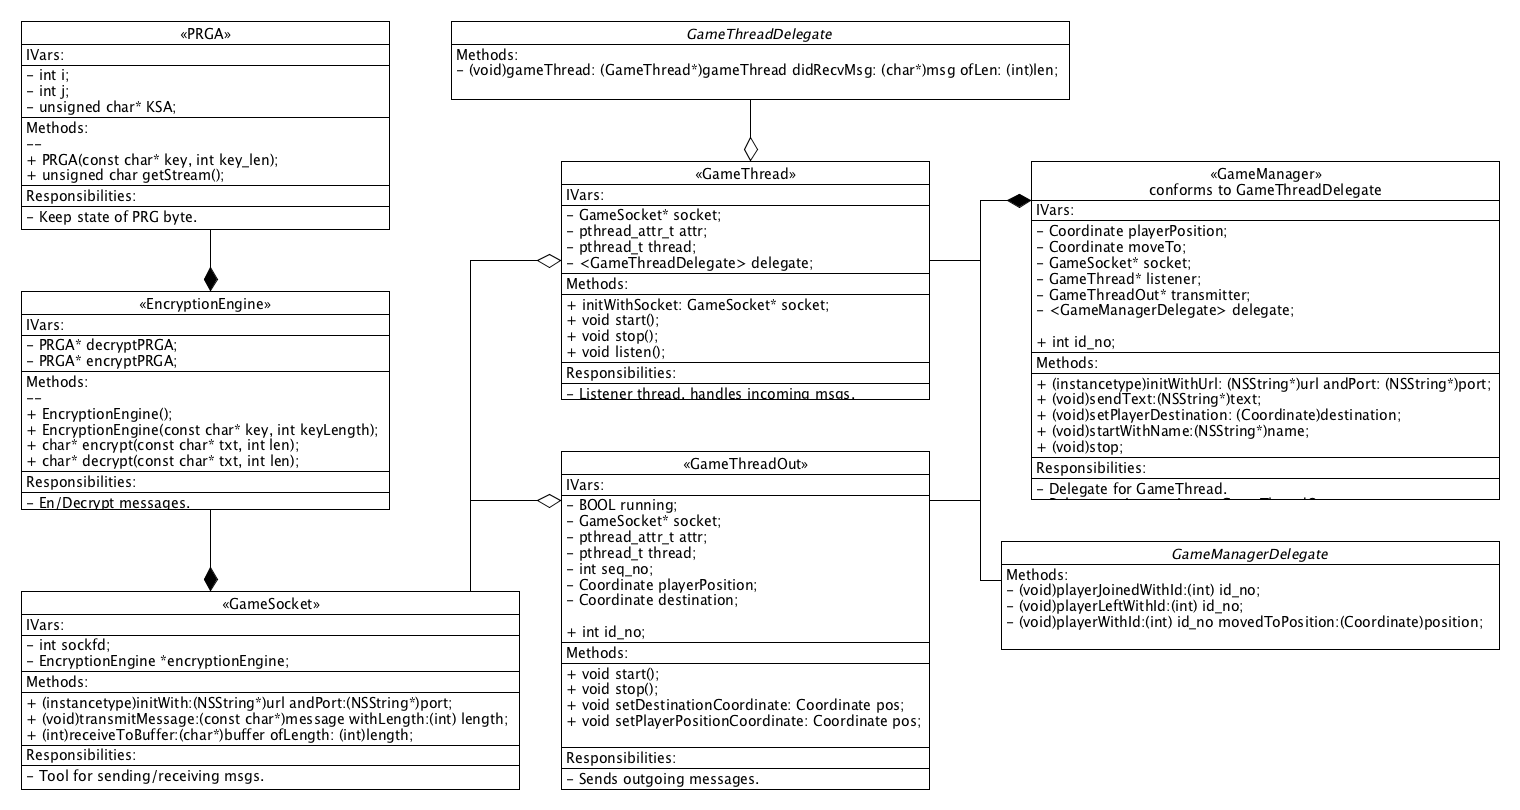
\includegraphics[scale=.2]{./png/ClientClassDiagram.png}			
		\end{center}
		\subsubsection{GameSocket}
		Innehåller metoder för att skicka och ta emot meddelanden av given form. Abstraherar berkeley socket APIn till för att göra det enkelt för ägare att använda klassen. Har en EncryptionEngine medlem som krypterar/dekrypterar alla meddelanden som passerar.
		\subsubsection{GameThreadOut}
		Tråd som sköter skickande av meddelanden till servern. När spelaren trycker på en punkt på skärmen så kommer denna tråd att skicka MoveEvent's tills dess att spelaren hamnar på denna position. I iOS måste main-tråden vara ledig för användning ty det är den som måste användas om någonting skall ritas på skärmen annars hade man kunnit låta main-tråden sköta alla ut-meddelanden.
		
		\newpage
		\subsubsection{GameThread}
		Lyssnar-tråd som delegerar mottaget meddelande till GameManager klassen.
		\subsubsection{GameManager}
		Delegat till GameThread. Initierar trådar och delegerar inkomna meddelanden till GameViewController.
		\subsubsection{GameViewController}
		Delegat till GameManager, klass som tar input från användaren och ritar ut spelarna på skärmen. Denna klass ärver från apple's (UIKit framework) UIViewController och  måste användas om man skall göra en iOS-applikation.
		
		\newpage
		\subsection{Server}
		\begin{center}
			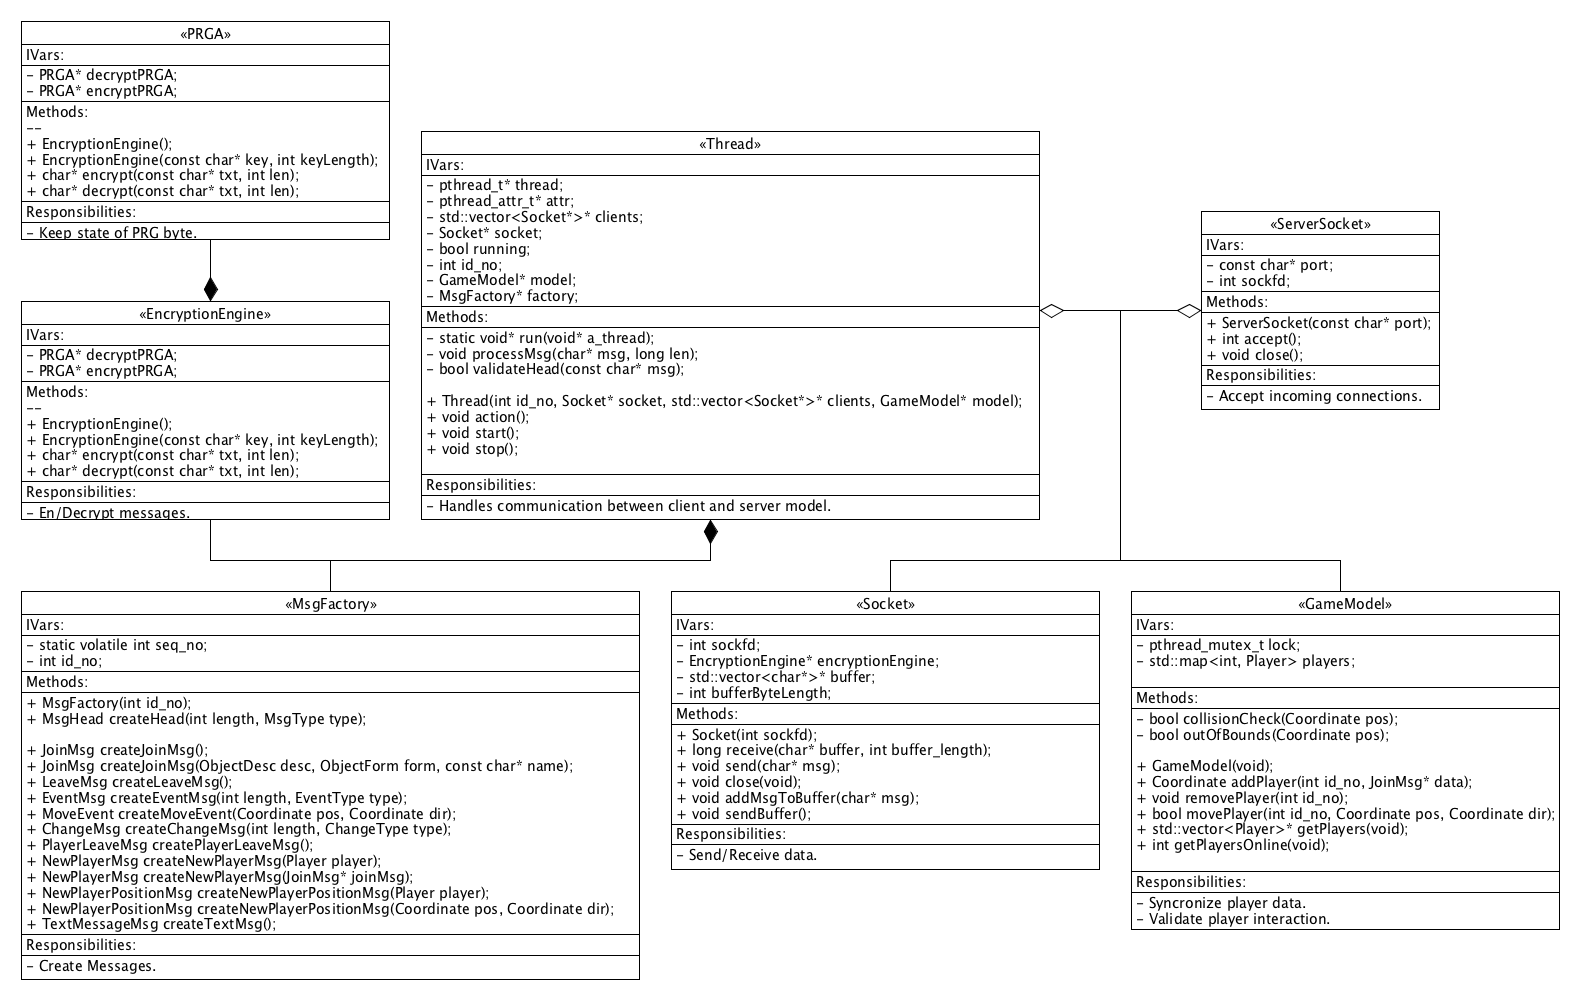
\includegraphics[scale=.2]{./png/ServerClassDiagram.png}			
		\end{center}
		\subsubsection{ServerSocket}
		När man instansierar en ServerSocket måste man ange det port-nummer man vill starta servern på i konstruktorn. Är angivet portnummer ledigt så kommer ServerSocket att köra:
			\begin{enumerate}
				\item getAddrInfo(): För att ta reda på vilken adress som servern befinner sig på.
				\item socket(): För att få ett socket file descriptor nummer som resterande metoder hänvisar till.
				\item bind(): För att binda till en adress, detta måste man göra för att kunna köra accept().
				\item listen(): Förbereder socket för inkommande trafik.
			\end{enumerate}
			
		När man nu har en ServerSocket så finns en metod ServerSocket::accept() som returnerar en Socket när en klient har anslutit.
		\subsubsection{Socket}
		Klass som abstraherar skickande och mottagande av meddelanden. Man kan skicka meddelanden ett och ett eller fylla en buffert med flera meddelande som kan skickas som ett meddelande.
		
		\subsubsection{Thread}
		Var ansluten klient får en egen tråd av serverns main funktion. Klassen Thread tar emot inkommande trafik från klienter och behandlar detta. Svarar sedan med ett unicast/multicast meddelande. Detta blockerar tråden för inkommande trafik men det spelar ingen roll då inkommande meddelanden sker i sekvens.
		
		\subsubsection{GameModel}
		Instansierad i main-funktionen på servern och delges till varje tråd så att de delar samma modell. Har metoder för att lägga till / ta bort / flytta spelare samt validera dessa. Åtgång till denna instans sker synkroniserat med hjälp av en mutex(Mutual Exclusion) referens.
		
		\subsubsection{MsgFactory}
		Klass som används för att skapa de meddelanden som servern skickar ut. Vid instansiering anger man id-nummer till konstruktorn så att de meddelanden som skapas har korrekt id. 
		
		\subsection{Kryptering}
		
	\section{Diskussion}%behandlar dina åsikter om Laborationen och vad du lärt dig.
  
    
\end{document}
